
%% [Afternoon beam broadening ]
%%________________________________________________________
\section{\Afternoon\ beam variations}% {\color{YellowGreen} Laurence}}
\label{se:obsdate_variations}

In this section, we evidence a beam size broadening depending on the
scan observation date. This effect, which mainly impacts late
afternoon observations and is reproducible from a campaign to another,
is probably due to deformations of the main dish subject to the Sun
heating. This is a well-known effect, which also impacts EMIR and was
observed for the previous generation of instrument MAMBO. However,
compared to the period when MAMBO or NIKA were on activity, these
daily deformations have probably strengthen due to the ageing of the
main dish white coating. \new{On short time scales, anomalous refraction
may also play a role~\cite{Altenhoff1987}. Based on observation
experience with EMIR, afternoon hours were
often impaired with an unstable atmosphere while rising moist air that
moves through the beam of the telescope causes the telescope beam
position to change within few seconds by several
arcseconds.}


\subsection{Beam monitoring using bright source scans}
\label{se:beam_monitoring_otf}

We monitor the time-dependent beam-size variations using all the
available bright source scans acquired at the optimal focus for each
campaign. Bright sources are selected by thresholding the flux density
estimates above $1\,\rm{Jy}$ at both wavelengths.
The beam size is estimated by fitting a 2D Gaussian from the map and
taking the geometrical FWHM, defined as 
$\rm{FWHM}_{\rm{geom}} = (\rm{FWHM}_x \rm{FWHM}_y)^{1/2}$, where
$\rm{FWHM}_x$ and $\rm{FWHM}_y$ are the best-fitting values of FWHM
along the minor and major axis of the elliptical 2D Gaussian.
% see def of RESULT_FWHM in nk_grid2info.pro line 320
% + see def of params in nika_gauss2d.pro
For Uranus, the FWHM estimates are corrected for the beam broadening due
to the finite extension of the apparent disc, as in Sect.~\ref{se:MB}. 

\begin{figure}[ht!]
  \begin{center}
    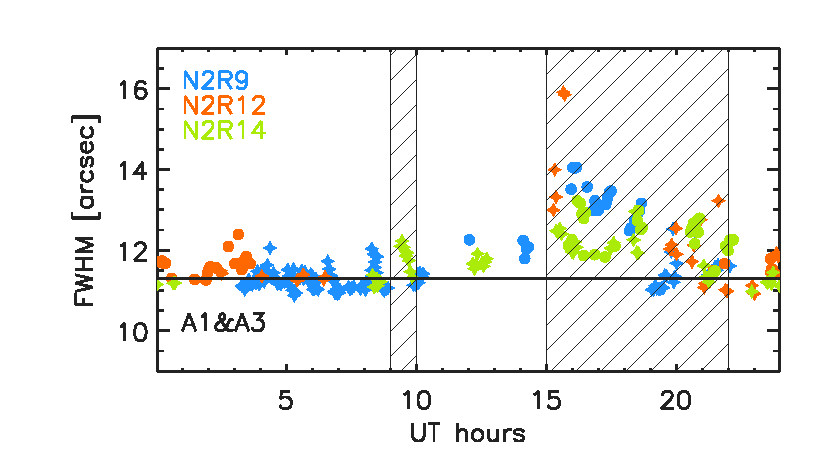
\includegraphics[clip=true, trim={0.9cm, 0.5cm, 0.5cm, 0.5cm}, width=0.4725\textwidth]{Figures/Beams/Beam_monitoring_with_otfs_vs_ut_1mm.pdf}
    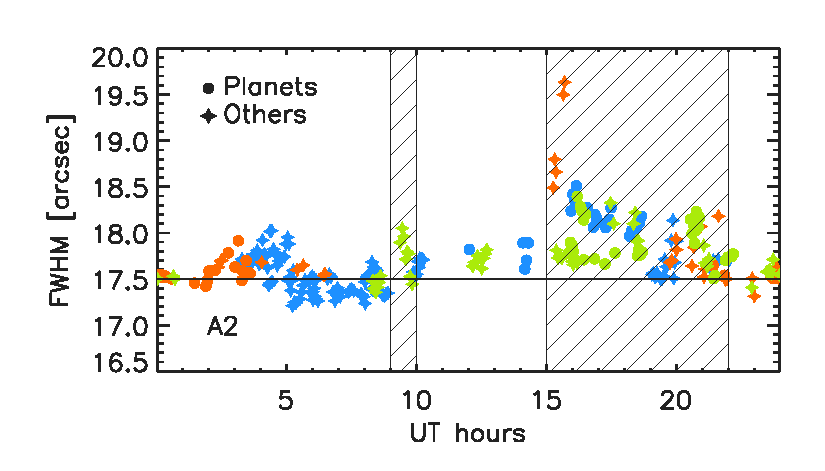
\includegraphics[clip=true, trim={0.5cm, 0.5cm, 0.5cm, 0.5cm}, width=0.4875\textwidth]{Figures/Beams/Beam_monitoring_with_otfs_vs_ut_a2.pdf}
    \caption[Beam size monitoring using OTF scans]{Beam size
      monitoring using OTF scans. FWHM at $1\,\rm{mm}$ (left panel)
      and $2\,\rm{mm}$ (right panel) as a function of the
      observation time in UT hours are shown using scans of giant
      planets (filled circles) and bright point-like sources above
      $1\,\rm{Jy}$ (filled stars) for N2R9 commissioning campaign and
      N2R12 and N2R14 science pools. The cross-hatched areas
      correspond to observing time period that are discarded using
      the baseline selection, as decribed in Sect.~\ref{se:data_selection}.} 
\label{fig:beam_monitoring_otf}
  \end{center}
\end{figure}

Figure~\ref{fig:beam_monitoring_otf} shows the geometrical FWHM as a
function of the observing time of the scans in UT hours for all OTF
scans of bright sources for the N2R9 commissioning campaign as well
as for the N2R12 and N2R14 science pools. For the three campaigns, we
observe the same evolution of the FWHM, which goes from a plateau at a
median value of $11.3''$ at $1\,\rm{mm}$ and $17.5''$ at $2\,\rm{mm}$
during the night, to a smooth rise that reaches a maximum of about $14''$
at $1\,\rm{mm}$ and $18.5''$ at $2\,\rm{mm}$ around 16:00 UT
hours. The beam broadening begins to become sizable around 15:00 UT
and one has to wait until around 22:00 UT for the beam sizes to lay
down on the stability plateau. The UT time ranges that are discarded
using the baseline scan selection (see
Sect.~\ref{se:data_selection}) are shown as cross-hatched areas in
Fig.~\ref{fig:beam_monitoring_otf}. They correspond to the afternoon
period between 15:00 and 22:00 UT hours, that is when the
telescope main dish is heated by daylight, as well as the
9:00-to-10:00 Sun rising period. The same beam size variations in time
using scans of giant planets (Uranus and Neptune) or other bright
sources (mainly quasars) are observed. However, FWHM from planets
observation tend to be slightly larger than FWHM from the observation
of other sources. This originates from larger 2D Gaussian fitted
values due to the error beams, which are measured with a
signal-to-noise as higher so as the source is bright. This small
effect is accounted for the beam-dependent calibration cross-check
discussed in Sect.~\ref{se:photocorr_calibration}.



\subsection{Beam monitoring using pointing}
\label{se:beam_monitoring_pointing}

As discussed in Sect.~\ref{se:pointing}, the telescope pointing is
monitored on a hour basis during observation using pointing
scans. However, as they consist of two sub-scans in azimuth and
elevation of about 10 seconds of integration time each, pointing scans
can be used to make a map of the pointing source. For each campaign,
we thus have on hand hundreds of maps of mostly point-like bright
sources. These can be also used to monitor the beam size\new{, although we
expect less accuracy than using standard bright source scans due to the
shorter integration time and the fact that only the centermost KIDs in
the array see the source.}  

%traitement pointing scans
For this purpose, pointing scans are reduced using
the data analysis pipeline described in
Sect.~\ref{se:pipeline_overview} with the same parameters as for
standard OTF scans, and projected onto maps of $2''$ resolution.
As previously, an elliptical 2D Gaussian is then fitted from the map
and a geometrical FWHM is formed from the best-fitting FWHM along the
two ellipse radii. FWHM estimates on Uranus maps are corrected for an
offset due to the finite size of the apparent disc, as discussed in
Sect.~\ref{se:beam_monitoring_otf}. Pointing scans on other extended
sources, such as NGC7027, are discarded from the analysis.

% anomalous refraction
\new{For each pointing, we also seek for anomalous refraction. There are
enough KIDs per observation band to make an independent map using only
one subscan, i.e. 10 seconds of integration time.
For each of the four cross subscans, we thus estimate the position of the best
2D Gaussian that fits the map. We compute the deviation between each
subscan-derived position and the best-fit position using the entire
scan. An anomalous refraction event is detected when the deviation is
above $2.5''$ for at least one subscan. We find that the apparent beam
broadening during afternoons is due to anomalous refraction for
between one third and one half of the scans\footnote{See the study posted
  in the commissioning internal wiki at
  \url{http://www.iram.fr/wiki/nika2/index.php/Millimetric_anomalies_(weather,_antenna)_as_monitored_by_pointing_scans}}.
} 

In Fig.~\ref{fig:beam_monitoring_pointing}, we present the FWHM
estimates using pointing scans as a function of the observing time in
UT hours for three observation campaigns. We observe the same beam
size evolution with UT hours as previously discussed in
Sect.~\ref{se:beam_monitoring_otf}, that is a plateau during night-time
and a smooth increase during day-time up to a maximum in the
afternoon, which is followed by a smooth decrease down to the plateau
a few hours after the sunset. Although the general trend is the same
as the OTF-based FWHM variations, more dispersion is seen either using
pointings toward giant planets or other bright sources.
%
\begin{figure}[ht!]
  \begin{center}
    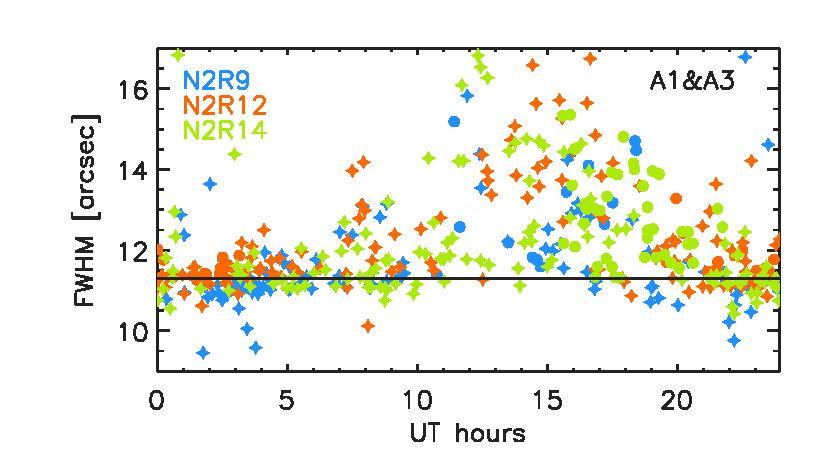
\includegraphics[clip=true, trim={0.9cm, 0.5cm, 0.5cm, 0.5cm}, width=0.4725\textwidth]{Figures/Beams/Beam_monitoring_with_pointings_vs_ut_1mm.pdf}
    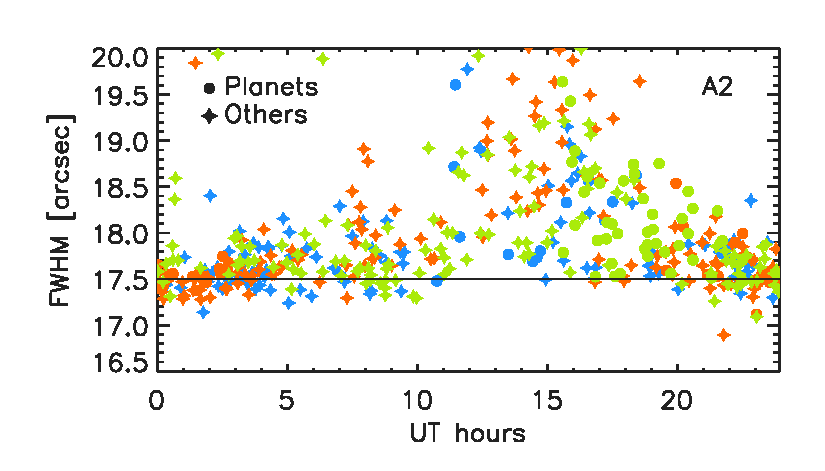
\includegraphics[clip=true, trim={0.5cm, 0.5cm, 0.5cm, 0.5cm}, width=0.4875\textwidth]{Figures/Beams/Beam_monitoring_with_pointings_vs_ut_a2.pdf}
    \caption[Beam size monitoring using pointing scans]{Beam size
      monitoring using pointing scans. Same legend as in
      Fig.~\ref{fig:beam_monitoring_otf}.} 
\label{fig:beam_monitoring_pointing}
\end{center}
\end{figure}
%
The pointing-based FWHM constitute a time-sampling of the FWHM during
the whole observation campaign. They can serve to estimate the beam
size of any observation scans, in particular
toward sources too faint for a direct FWHM fit to be made on the
projected map. To mitigate the dispersion, the time-stamped
pointing-based FWHM is filtered with a running median on a 70-minute
width time window. Then, the FWHM at the time of the considered scans is
interpolated from the smoothed pointing-based time-stamped FWHM.
%
\begin{figure}[ht!]
  \begin{center}
    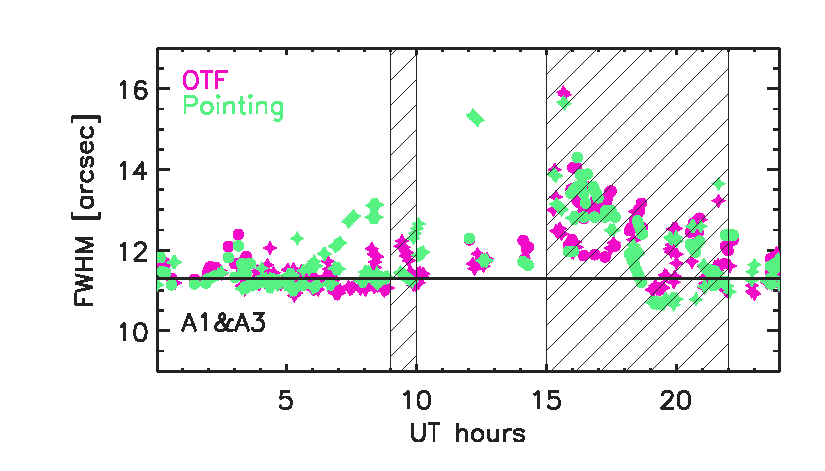
\includegraphics[clip=true, trim={0.9cm, 0.5cm, 0.5cm, 0.5cm}, width=0.4725\textwidth]{Figures/Beams/Beam_monitoring_with_otfs_vs_ut_compare_pointings_1mm.pdf}
    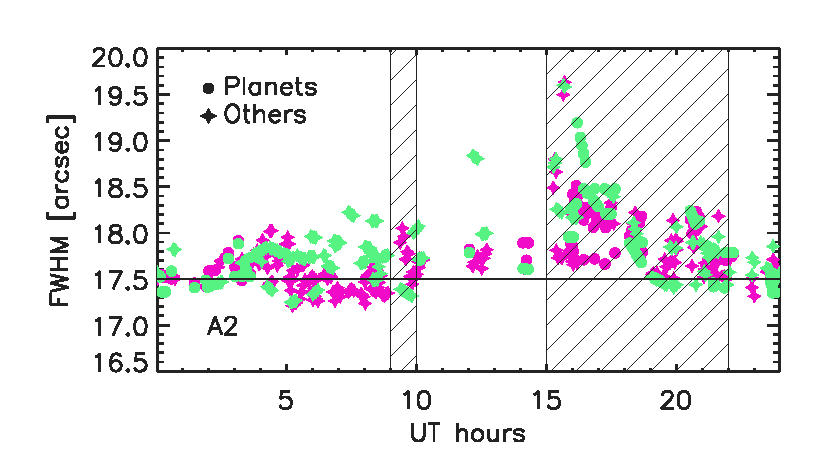
\includegraphics[clip=true, trim={0.5cm, 0.5cm, 0.5cm, 0.5cm}, width=0.4875\textwidth]{Figures/Beams/Beam_monitoring_with_otfs_vs_ut_compare_pointings_a2.pdf}
    \caption[Beam size monitoring comparison]{Beam size monitoring
      comparison. The FWHM estimates from a 2D Gaussian fit on the map
      of OTF scans toward bright sources ('OTF'-labeled pink data
      points) are compared to FWHM estimates that are obtained by
      interpolating the smoothed pointing-based FWHM at the time of
      the scans ('Pointing'-labeled light green data points).}
\label{fig:beam_monitoring_compare}
\end{center}
\end{figure}
%
Figure~\ref{fig:beam_monitoring_compare} shows two different FWHM
estimates for the same data set: the best-fitting FWHM estimates on
the map are compared with the interpolation from the pointing-based
FWHM monitoring. The two estimates are well in agreement with each
other, although the pointing-based estimates have more dispersion and
a few outliers.\\

As a summary, we have evidenced a systematic beam size variation with
the observation time using two different data sets: a series of OTF
scans of bright sources and pointing scans. The beam size
variation is i) reproducible from a campaign to another, stable
with ii) the data set and iii) the sources. It consists of a beam
broadening during afternoons and an increase of the dispersion during
sunrises. \new{The \afternoon\ beam-size variation effect mainly
originates from deformations of the $30\,\rm{m}$ primary mirror subject
to the Sun irradiation, while anomalous refraction also play a
role.}  
The most impacted
observing periods are well discarded using the baseline selection
criteria discussed in Sect.~\ref{se:data_selection}.


